{\textbf{1. 概念}}

{散列表就是根据给定的关键字来计算出关键字在表中的地址。}

{\textbf{2. 构造}}

{常用的Hash函数的构造方法}

{(1)直接定址法}

{~即H(key)=key或H(key)=a*key+b}

{(2)数字分析法}

{假设关键字是r进制,并且Hash表中可能出现的关键字都事先知道,则去关键字的若干位数组成散列地址。}

{(3)平方取中法}

{取关键字平方后的中间几位为散列地址。}

{(4)除留余数法}

{即H(key)=key mod
p,{一般p选择小于或者等于表长的最大素数},这样可以减少冲突。}

{\textbf{3. 冲突处理}}

{冲突:因为Hash函数的关系,常常会发生多个关键字共用一个地址的情况,这种情况就称为冲突。冲突处理就是为共用一个地址的关键字找到另一个``空''的散列地址。}

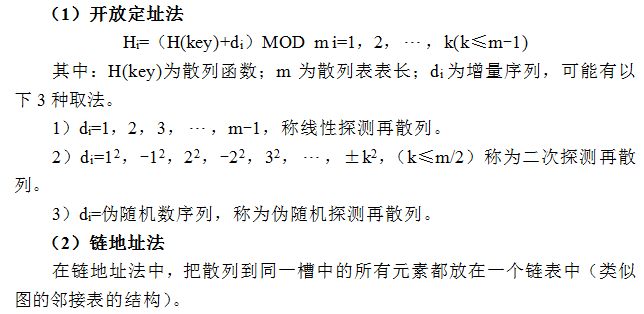
\includegraphics[width=3.70833in,height=1.81250in]{png-jpeg-pics/AB38936DEDE13BE2CB95F5C0E3081756.png}

{\textbf{4. 性能分析}}

{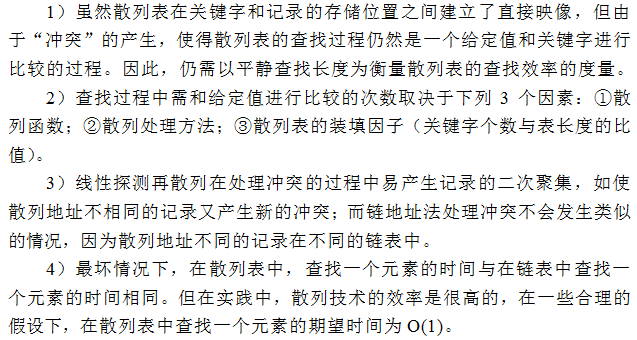
\includegraphics[width=3.70833in,height=1.97917in]{png-jpeg-pics/9716B27691E0F50D520BD597E56948C0.png}}
